\documentclass{article}

\usepackage[eandd]{neurips_2026}

\usepackage[utf8]{inputenc}
\usepackage[T1]{fontenc}
\usepackage{hyperref}
\usepackage{url}
\usepackage{booktabs}
\usepackage{amsfonts}
\usepackage{nicefrac}
\usepackage{microtype}
\usepackage{xcolor}
\usepackage{graphicx}
\usepackage{array}
\usepackage{tabularx}
\usepackage{tikz}
\usepackage{enumitem}

\definecolor{roleref}{HTML}{2C5F8A}
\definecolor{rolecanon}{HTML}{3A7D44}
\definecolor{roleexpl}{HTML}{CC7722}
\definecolor{rolediag}{HTML}{999999}

\newcolumntype{L}[1]{>{\raggedright\arraybackslash}p{#1}}
\newcolumntype{Y}{>{\raggedright\arraybackslash}X}

\title{Benchmarking Paired fMRI Perception--Imagery Decoding\\Under Overlap Scarcity}

\author{Anonymous Authors}

\begin{document}

\maketitle

% ==========================================================================
%  ABSTRACT
% ==========================================================================
\begin{abstract}
Paired perception--imagery decoding from fMRI is scientifically important but
evaluation-poor.  When perception and imagery sessions share only a handful of
overlapping stimuli, the question shifts from \emph{which decoder is best?}\ to
\emph{which conclusions are even warranted?}  We contribute a frozen benchmark
and evaluation surface for this overlap-scarce regime---not a new decoder
architecture.  The benchmark comprises 94 mixed rows, 5 shared paired stimulus
identifiers, and 1 held-out paired evaluation group across four subjects from
the Natural Scenes Dataset.  We evaluate a fixed comparison ladder of three
decoder families: Ridge regression (external low-data reference), a shared-only
neural decoder (canonical neural baseline), and shared-private neural variants
(exploratory hypothesis family).  On this surface, Ridge is the strongest
overall baseline (test cosine similarity 0.552, test MSE 0.00117), shared-only
is the strongest canonical neural model (0.136, 0.00225), and the best
shared-private variant remains below shared-only (0.108, 0.00232).  These
results yield a deliberately qualified conclusion: the current evidence does not
support explicit disentanglement as the preferred model family under severe
overlap scarcity.  We are not aware of a prior frozen benchmark for paired
perception--imagery decoding under explicit overlap constraints, or one that
pre-declares evidential roles before evaluation.  The contribution is therefore
a frozen evaluation surface with pre-declared model roles, a reusable
comparison ladder, and a claim-boundary methodology documenting which
conclusions the current regime does and does not support.  Future studies with
larger paired data can rerun the same protocol without changing the evaluation
contract.
\end{abstract}

% ==========================================================================
%  1. INTRODUCTION
% ==========================================================================
\section{Introduction}

The central bottleneck in paired perception--imagery brain decoding is not
architectural: it is evaluative.  When the number of stimuli shared between
perception and imagery sessions is extremely small, standard model comparisons
become fragile, held-out evaluation sets shrink to the point of unreliability,
and more expressive architectures become easy to overinterpret.  This
\emph{overlap scarcity} problem is not a local inconvenience in one particular
dataset.  It is a structural feature of realistic paired neuroimaging settings,
where the intersection between externally driven and internally generated
responses is filtered through subject availability, stimulus overlap, and split
constraints
\citep{pearson2019imagery,horikawa2017generic,dijkstra2018temporal}.

Despite this, much recent fMRI decoding work has focused on architectural
sophistication or reconstruction quality rather than on whether evaluation
surfaces actually support the conclusions drawn from them
\citep{takagi2023high,radford2021clip}.  This creates a particular risk in
paired perception--imagery settings, where shared-private or disentangled models
carry an appealing narrative---that perception and imagery can be factored into
shared content and domain-specific components---but that narrative requires
sufficient paired evidence to justify.  When paired supervision is scarce,
transfer diagnostics become fragile, held-out support is narrow, and expressive
models become easy to overinterpret.  A conceptually attractive shared-private
model may still be empirically unjustified if it is evaluated on too little
paired data or against an insufficiently disciplined baseline ladder.

This paper treats evaluation discipline as the primary contribution rather than
model novelty.  We freeze a benchmark, report the current model ordering
honestly, and document the claim boundary that the present paired regime
supports.  The benchmark is real but severely constrained: 94 mixed rows across
four subjects, with only 5 shared paired stimulus identifiers and 1 held-out
paired evaluation group.  On this surface, Ridge regression is the strongest
overall baseline, a shared-only neural decoder is the strongest canonical neural
model, and shared-private variants remain exploratory.

We argue that this is a useful contribution to the NeurIPS Evaluations and
Datasets track for three reasons.  First, no frozen benchmark surface currently
exists for paired perception--imagery decoding under overlap scarcity.
Researchers who wish to compare models in this regime must build ad hoc
evaluations whose data regime, target space, and baseline roles vary between
studies---precisely the kind of benchmark fragility that
\citet{dehghani2021benchmark} showed can reverse model rankings in other
domains.  Second, the benchmark's qualified findings directly prevent a concrete
failure mode: without a stable reference ladder, future work may attribute
neural-model gains to disentanglement rather than to changes in dataset scale,
because no fixed comparison point exists.  Third, the evaluation protocol is
designed for reuse.  Its pre-declared evidential roles and fixed target space
mean that when larger paired overlap becomes available, the same ladder can be
rerun and directly compared to the current ordering without redesigning the
evaluation.

\paragraph{Contributions.}
\begin{itemize}[nosep,leftmargin=1.5em]
\item A reproducible ROI-first benchmark for multi-subject paired
  perception--imagery decoding, with canonical preparation, preflight,
  training, evaluation, and export workflows.
\item A frozen comparison ladder that assigns fixed evidential roles---external
  reference baseline, canonical neural baseline, exploratory hypothesis
  family---before interpretation begins.
\item An honest evidence report under severe overlap scarcity: Ridge is
  strongest overall, shared-only is the strongest canonical neural model, and
  shared-private disentanglement is not yet justified as the preferred family.
\item A frozen claim boundary that documents what can and cannot be concluded
  from the current benchmark, designed to prevent overclaiming and to
  motivate---but not confirm---a future threshold hypothesis.
\end{itemize}

\noindent
Absent this benchmark, the practical risk is concrete: paired
perception--imagery decoding would continue without a frozen comparison point.
Architectural conclusions would rest on evaluations whose data regime, target
space, and baseline roles vary between studies, making it impossible to
determine whether a reported improvement reflects genuine progress or a change
in evaluation conditions.  This benchmark does not solve the data-scarcity
problem.  It makes the problem legible and auditable, so that future work can
build on a stable foundation rather than on shifting sand.

% ==========================================================================
%  2. RELATED WORK
% ==========================================================================
\section{Related Work}

\paragraph{Visual content decoding from fMRI.}
Large-scale fMRI datasets such as the Natural Scenes Dataset
\citep{allen2022nsd}, BOLD5000 \citep{chang2019bold5000}, and THINGS-data
\citep{hebart2023things} have enabled rapid progress in visual content decoding.
Early deep-learning approaches demonstrated that hierarchical visual features
can be recovered from brain activity \citep{shen2019deep}, and recent
reconstruction systems leverage latent diffusion models and large pretrained
vision-language encoders to generate high-fidelity images from fMRI
\citep{takagi2023high,ozcelik2023brain,scotti2024mindeye2}.  These systems
achieve impressive perceptual quality but are evaluated almost exclusively on
perception-only decoding with abundant training data.
\citet{tang2023semantic} extended decoding to continuous language, further
raising expectations for what brain decoders can achieve.  Yet the harder paired
perception--imagery regime---where overlapping stimuli between conditions are
scarce---remains comparatively underserved in terms of evaluation discipline.

\paragraph{Perception--imagery transfer and disentanglement.}
\citet{horikawa2017generic} demonstrated that hierarchical visual features can
be decoded from both seen and imagined objects, establishing the basic
scientific question.  \citet{pearson2019imagery} and \citet{dijkstra2018temporal}
further characterized the neural overlap and divergence between perception and
imagery.  These studies motivate shared-private or disentangled modeling, but
the datasets available for such modeling are typically small, evaluation
surfaces have not been frozen in a way that separates architectural conclusions
from data-support limitations, and no prior work has pre-declared the
evidential roles of competing model families before reporting paired results.

\paragraph{Benchmark methodology.}
The broader ML community has recognized that benchmark design itself is a
source of fragility.  \citet{dehghani2021benchmark} showed that relative model
rankings can change substantially depending on which evaluation tasks are
included, underscoring the importance of fixing the evaluation surface before
drawing architectural conclusions.  Large-scale holistic evaluations
\citep{liang2023helm} have demonstrated the value of standardized, transparent
comparison ladders across diverse tasks.  Our contribution applies a similar
principle to a much smaller but structurally important domain: paired
perception--imagery fMRI decoding, where no standardized evaluation surface
currently exists.

\paragraph{Multi-subject alignment.}
\citet{naselaris2011encoding} emphasized principled encoding and decoding
comparisons, and multi-subject alignment methods \citep{haxby2011hyperalignment}
have shown that representational comparisons require careful normalization.  Our
benchmark adopts an ROI-first input contract rather than voxel-wise alignment,
which is sufficient for the comparison-ladder question addressed here.

% ==========================================================================
%  3. BENCHMARK DESIGN
% ==========================================================================
\section{Benchmark Design}

The scientific object in this paper is a paired benchmark under constrained
support.  We study a regime in which perception and imagery are aligned through
a shared stimulus identifier, but only for a very small set of paired items.

\paragraph{Data regime and overlap scarcity.}
The benchmark is derived from the intersection of two public neuroimaging
resources: canonical perception indices from the Natural Scenes Dataset
\citep{allen2022nsd} and mental imagery response data from the public
NSD-Imagery acquisition.  After canonical filtering, overlap assembly, and
multi-subject intersection, the resulting prepared dataset contains 94 rows
across subjects \texttt{subj02} (38 rows), \texttt{subj03} (18),
\texttt{subj05} (19), and \texttt{subj07} (19), with 5 shared paired stimulus
identifiers and 1 held-out paired evaluation group.

This scarcity is not an artifact of poor data engineering.  It reflects a
genuine ceiling on the overlap between currently accessible perception and
imagery sessions after principled filtering.  The benchmark's checked-in
preflight policy classifies this as below \emph{confirmatory} paper-scale
readiness (which requires $\geq\!32$ paired groups for strong positive claims
about disentanglement).  We report this threshold transparently and treat the
benchmark accordingly: it is appropriate for freezing a comparison ordering and
documenting a claim boundary, but not for strong confirmatory statements.  The
gap between the threshold and the current data is itself an important finding:
it quantifies how much more paired support the community needs before
shared-private conclusions become defensible.

\paragraph{Fixed target space and input contract.}
Every model in the ladder predicts the same target representation,
\texttt{vit\_l14\_image\_768}, so the benchmark compares decoder structure
rather than target-space drift.  The multi-subject input contract is ROI-first:
fMRI features are organized into three ROI groups---early visual, ventral
visual, and metacognitive---rather than raw full-fMRI vectors.  This is
consistent with representational rather than voxel-wise multi-subject alignment
\citep{haxby2011hyperalignment} and necessary for valid multi-subject batching
across subjects with different raw voxel dimensionalities.

\paragraph{Readiness and scope.}
Overlap scarcity matters for three reasons, each specific to the paired
perception--imagery setting rather than to low-data regimes in general.  First,
it limits what can be inferred from held-out \emph{paired} evaluation: a small
number of paired groups makes transfer-like claims and domain-specific
diagnostics inherently weak, in a way that single-domain scarcity does not.
Second, it changes the burden placed on model capacity asymmetrically: when
paired supervision is sparse, shared-private factorizations pay a capacity
penalty that shared-only or linear models do not, because the private branches
must be justified by paired evidence that may not exist.  Third, it increases
the importance of comparison discipline: if data preparation, target spaces, or
model roles drift between baselines, the benchmark stops answering the intended
scientific question about shared versus private structure.

% ==========================================================================
%  4. COMPARISON LADDER AND EVALUATION PROTOCOL
% ==========================================================================
\section{Comparison Ladder and Evaluation Protocol}

The benchmark assigns fixed evidential roles to each model family
\emph{before} interpretation.  This pre-declaration is a deliberate
methodological choice: when a comparison surface is small, post-hoc role
reassignment (e.g., reclassifying a failed primary model as a ``diagnostic
control'') can disguise negative results as designed ablations.  By fixing
roles in advance, the benchmark preserves the scientific meaning of the
ordering regardless of which model wins.

\paragraph{Model roles.}
\emph{Ridge regression} is the external low-data reference baseline.  Simple
linear models remain strong comparators in fMRI decoding
\citep{naselaris2011encoding}, and Ridge serves as an honest floor: if an
expressive neural model cannot beat Ridge under scarce overlap, the
architectural complexity is not yet warranted.  \emph{Shared-only} is the
canonical neural baseline.  It uses the same ROI-first input and target space as
the shared-private family but removes explicit private branches and domain
classification, providing the simplest neural comparator.  \emph{Shared-private
variants} are the exploratory hypothesis family.  They carry the heaviest burden
of proof: a more expressive factorization requires evidence that it helps rather
than simply fits the task narrative.  Three shared-private variants are
evaluated: the default model, a reduced-capacity variant with
\texttt{private\_dim=16}, and a \texttt{private\_dim=8} recovery variant.  A
no-domain-head ablation (shared-private with domain classification disabled) is
included as a diagnostic control.

\paragraph{Hyperparameters and metrics.}
All neural runs use the same checked-in hyperparameter family: batch size 8, 5
training epochs, learning rate $10^{-3}$, weight decay $10^{-4}$, and seed~0.
Primary metrics are content cosine similarity and content MSE on the held-out
evaluation set.  Condition-level imagery and perception means are reported where
present in the frozen evidence bundle.  Transfer summaries and domain accuracy
remain secondary diagnostics only: with 1 held-out paired group they are too
weak to sustain a headline claim.

\begin{table}[t]
  \centering
  \footnotesize
  \caption{Frozen comparison ladder on the max-available paired overlap set
  (94 rows, 5 shared paired IDs, 4 subjects).
  Bold marks the best value in each metric.  Dashes indicate condition-level
  means absent from the frozen evidence bundle.  ``Groups'' is the number of
  held-out paired evaluation groups.  Evidential roles are pre-declared.}
  \label{tab:results}
  \begin{tabularx}{\linewidth}{@{}L{2.0cm}Ycc@{\hspace{6pt}}c@{\hspace{6pt}}cc@{}}
    \toprule
    System & Evidential role & Cosine\,$\uparrow$ & MSE\,$\downarrow$ &
      Img.\ mean & Perc.\ mean & Groups \\
    \midrule
    Ridge
      & External low-data reference
      & \textbf{0.55199} & \textbf{0.001167}
      & 0.55152 & 0.55446 & 1 \\[2pt]
    Shared-only
      & Canonical neural baseline
      & 0.13596 & 0.002250
      & 0.13422 & 0.14527 & 1 \\
    \addlinespace[4pt]
    \multicolumn{7}{@{}l}{\textit{Exploratory shared-private family}} \\
    \addlinespace[2pt]
    \hspace{0.3em}SP, $d_\mathrm{priv}\!=\!16$
      & Best SP variant tested
      & 0.10784 & 0.002323
      & --- & --- & 1 \\
    \hspace{0.3em}SP, $d_\mathrm{priv}\!=\!8$
      & Recovery variant
      & 0.09595 & 0.002354
      & --- & --- & 1 \\
    \hspace{0.3em}SP default
      & Hypothesis-family baseline
      & 0.06927 & 0.002424
      & 0.07151 & 0.05735 & 1 \\
    \hspace{0.3em}SP, no domain head
      & Diagnostic control
      & 0.05907 & 0.002450
      & --- & --- & 1 \\
    \bottomrule
  \end{tabularx}
\end{table}

% ==========================================================================
%  5. RESULTS
% ==========================================================================
\section{Results}

The main result is a benchmark ordering, not a model novelty claim.
Table~\ref{tab:results} reports the frozen ladder.  We organize the findings
into three tiers by evidential strength.

\paragraph{Strongly supported findings.}
First, the ROI-first benchmark is operational on real paired data and produces a
stable, reproducible comparison ladder.  Second, within the present low-overlap
regime, simpler models dominate.  Ridge is the strongest overall baseline (test
cosine 0.55199, test MSE 0.001167), and shared-only is the strongest canonical
neural model (0.13596, 0.002250).  The gap between Ridge and all neural models
is large, indicating that linear regression remains a formidable comparator when
paired training data is severely limited.

\paragraph{Diagnostic findings.}
The shared-private story is more limited but still informative.  Reducing
private capacity helps within that family: both \texttt{private\_dim=16}
(0.10784) and \texttt{private\_dim=8} (0.09595) improve over the default
shared-private model (0.06927).  However, none overtakes shared-only.  Disabling
the domain head alone does not rescue shared-private performance (0.05907),
suggesting that the gap is not attributable to a single broken auxiliary
component.  Instead, the pattern is consistent with a scarce-overlap regime that
penalizes unnecessary capacity, regardless of where that capacity sits.

\paragraph{Unsupported conclusions.}
The current results do not show that shared-private disentanglement improves
content decoding.  They do not show that shared-private structure improves
transfer generalization.  They do not show that private branches already isolate
neuroscientifically meaningful perception-private or imagery-private factors.
And they do not confirm a threshold at which disentanglement begins to help.

\begin{figure}[t]
  \centering
  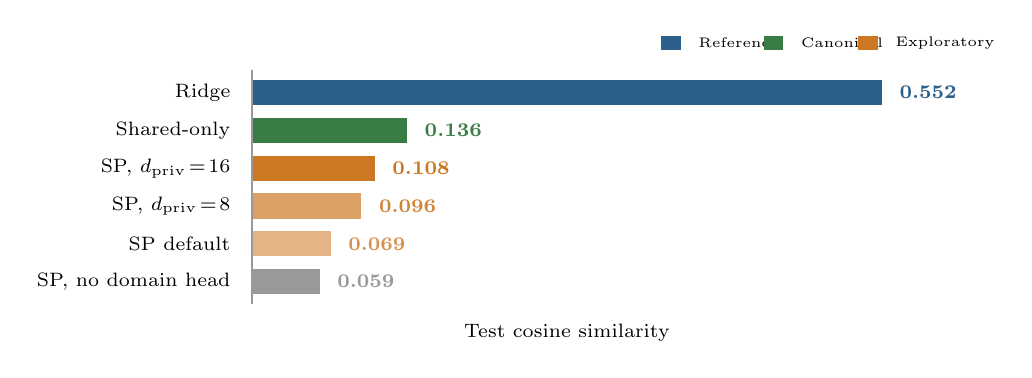
\begin{tikzpicture}
    \fill[rolediag] (0,0) rectangle (0.86,0.32);
    \node[anchor=east, font=\scriptsize] at (-0.15, 0.16)
      {SP, no domain head};
    \node[anchor=west, font=\scriptsize\bfseries, text=rolediag]
      at (0.96, 0.16) {0.059};

    \fill[roleexpl!55] (0,0.48) rectangle (1.00,0.80);
    \node[anchor=east, font=\scriptsize] at (-0.15, 0.64)
      {SP default};
    \node[anchor=west, font=\scriptsize\bfseries, text=roleexpl!80]
      at (1.10, 0.64) {0.069};

    \fill[roleexpl!70] (0,0.96) rectangle (1.39,1.28);
    \node[anchor=east, font=\scriptsize] at (-0.15, 1.12)
      {SP, $d_\mathrm{priv}\!=\!8$};
    \node[anchor=west, font=\scriptsize\bfseries, text=roleexpl!90]
      at (1.49, 1.12) {0.096};

    \fill[roleexpl] (0,1.44) rectangle (1.56,1.76);
    \node[anchor=east, font=\scriptsize] at (-0.15, 1.60)
      {SP, $d_\mathrm{priv}\!=\!16$};
    \node[anchor=west, font=\scriptsize\bfseries, text=roleexpl]
      at (1.66, 1.60) {0.108};

    \fill[rolecanon] (0,1.92) rectangle (1.97,2.24);
    \node[anchor=east, font=\scriptsize] at (-0.15, 2.08)
      {Shared-only};
    \node[anchor=west, font=\scriptsize\bfseries, text=rolecanon]
      at (2.07, 2.08) {0.136};

    \fill[roleref] (0,2.40) rectangle (8.0,2.72);
    \node[anchor=east, font=\scriptsize] at (-0.15, 2.56)
      {Ridge};
    \node[anchor=west, font=\scriptsize\bfseries, text=roleref]
      at (8.10, 2.56) {0.552};

    \draw[thin, black!40] (0,-0.12) -- (0, 2.85);
    \node[font=\scriptsize, anchor=north] at (4.0, -0.25)
      {Test cosine similarity};

    \fill[roleref]   (5.2,3.10) rectangle ++(0.25,0.18);
    \node[anchor=west, font=\tiny] at (5.55,3.19) {Reference};
    \fill[rolecanon] (6.5,3.10) rectangle ++(0.25,0.18);
    \node[anchor=west, font=\tiny] at (6.85,3.19) {Canonical};
    \fill[roleexpl]  (7.7,3.10) rectangle ++(0.25,0.18);
    \node[anchor=west, font=\tiny] at (8.05,3.19) {Exploratory};
  \end{tikzpicture}
  \caption{Frozen benchmark ladder on the max-available paired overlap set.
  Bar length is proportional to test cosine similarity.
  Ridge dominates all neural models; shared-only is the strongest
  canonical neural baseline; all shared-private (SP) variants remain
  below shared-only.  Color encodes the system's pre-declared evidential
  role.}
  \label{fig:ladder}
\end{figure}

\paragraph{Takeaway.}
The benchmark supports a disciplined ordering, not a crossover claim.  Ridge
remains the strongest reference point, shared-only is the correct current
neural baseline, and shared-private remains exploratory.  This is not a failed
method paper reframed as a benchmark: the benchmark was designed to determine
whether disentanglement is justified under scarce paired overlap, and the answer
is that it is not yet justified.  That qualified conclusion is the paper's
scientific contribution.

% ==========================================================================
%  6. DISCUSSION AND CLAIM BOUNDARY
% ==========================================================================
\section{Discussion}

\paragraph{What the benchmark establishes.}
The frozen benchmark establishes three things.  First, a reproducible evaluation
surface exists for paired perception--imagery decoding under overlap scarcity:
the preparation, training, evaluation, and comparison workflows are operational
and auditable.  Second, the current model ordering is clear and stable:
Ridge $>$ shared-only $>$ shared-private.  Third, several tempting architectural
conclusions are ruled out: explicit disentanglement does not improve content
decoding in this regime, shared-private structure does not improve transfer
generalization, and private branches do not yet capture neuroscientifically
interpretable structure.

\paragraph{What is suggestive but not confirmed.}
The pattern of improvement within the shared-private family as private capacity
decreases is consistent with the hypothesis that disentanglement may begin to
help only when paired support is large enough to sustain the additional
capacity.  This motivates a \emph{threshold hypothesis}---the idea that there
exists some overlap scale at which shared-private models cross above
shared-only---but the present evidence only motivates that hypothesis; it does
not confirm it.

\paragraph{Why negative findings matter for E\&D.}
Overclaiming is a persistent risk in brain decoding, where strong narratives
about what architectures ``should'' do can outrun the evaluation data.  Consider
the concrete failure mode this benchmark prevents: a future study might report
that a shared-private model improves paired decoding, but if that study uses a
different data regime, a different target space, or a different baseline ladder,
there is no way to tell whether the gain came from the architecture or from a
change in evaluation conditions.  A frozen benchmark with an honest ordering
makes this kind of confound detectable: the same ladder can be rerun under the
new conditions, and any performance change can be attributed to the data or
architecture rather than to benchmark drift.

\paragraph{Why this community, why now.}
The NeurIPS Evaluations and Datasets track is the right venue because the core
problem is evaluation methodology under data-support mismatch, not model
novelty.  \citet{dehghani2021benchmark} showed that benchmark design choices
can reverse model rankings; this work applies the same lesson to a setting
where no standardized benchmark exists at all.  The question of when benchmark
evidence is sufficient to support architectural conclusions is a general ML
concern, but it is especially acute in brain decoding, where paired supervision
is structurally scarce and strong narratives about shared-private factorization
can outrun the data.  This benchmark is timely because recent
reconstruction-focused work
\citep{takagi2023high,ozcelik2023brain,scotti2024mindeye2} has raised
expectations for what brain decoders can achieve, increasing the risk that
paired perception--imagery claims will be made without adequate evaluation
surfaces.

\paragraph{Reproducibility as contribution.}
The benchmark is tied to checked-in canonical configs, a fixed target space,
explicit workflow entry points, and named artifact roots for preparation,
training, evaluation, and export.  This matters because a negative or qualified
result is only informative if reviewers can see that the comparison surface was
disciplined rather than ad hoc.  The paper's main claims are grounded in four
artifact-bearing surfaces: the prepared mixed overlap dataset, the shared target
cache, the baseline/model artifact roots, and the preflight status that records
why the benchmark remains below paper-scale support.  Appendix~\ref{app:repro}
provides the config-command-artifact contract for the main stages.

\begin{table}[t]
  \centering
  \footnotesize
  \caption{Claim boundary for the frozen benchmark.  Each row classifies a
  potential conclusion and states what additional evidence would be needed
  to upgrade it.  The paper is strongest as an evaluation and reproducibility
  contribution, not as a positive disentanglement result.}
  \label{tab:claims}
  \begin{tabularx}{\linewidth}{@{}L{1.45cm}YY@{}}
    \toprule
    Status & Conclusion & Evidence needed to upgrade \\
    \midrule
    \textbf{Supported}
      & The benchmark provides a reproducible ROI-first evaluation surface for
        multi-subject paired perception--imagery decoding.
      & None; operational claim is validated. \\[3pt]
    \textbf{Supported}
      & Ridge is the strongest model on the current low-overlap benchmark.
      & None; frozen ordering on the current surface. \\[3pt]
    \textbf{Supported}
      & Shared-only is the strongest canonical neural baseline.
      & None; frozen ordering on the current surface. \\[3pt]
    Partial
      & Low-overlap regimes favor simpler decoders over explicit
        disentanglement.
      & Repeated evidence on larger paired datasets or controlled overlap
        sweeps. \\[3pt]
    Partial
      & Private-capacity scaling matters in low-data regimes.
      & More capacity settings and reruns on larger data. \\[3pt]
    \textit{Not justified}
      & Shared-private disentanglement improves content decoding.
      & Materially larger paired benchmark where SP beats shared-only. \\[3pt]
    \textit{Not justified}
      & The threshold hypothesis is confirmed.
      & Overlap-expansion study showing a transition in model ordering. \\[3pt]
    \textit{Not justified}
      & Private latents are neuroscientifically meaningful.
      & Larger paired support, stable ROI analyses, repeated evidence. \\
    \bottomrule
  \end{tabularx}
\end{table}

% ==========================================================================
%  7. THREATS TO VALIDITY
% ==========================================================================
\section{Threats to Validity}

We organize the main threats by source and then explain why they are compatible
with a valid E\&D contribution.

\paragraph{Overlap scarcity.}
The benchmark contains only 94 rows and 5 shared paired stimulus identifiers.
This is the primary limitation.  It means the results are adequate for freezing
a benchmark ordering and ruling out some stronger claims, but not for
establishing a general law about when disentanglement should help.  The
preflight policy classifies this regime as below paper-scale readiness (which
requires $\geq\!32$ paired groups).  We treat this limitation as part of the
contribution rather than as a weakness to hide: the overlap scarcity problem
itself is what the benchmark makes legible.

\paragraph{Held-out support weakness.}
With only 1 held-out paired evaluation group, transfer diagnostics and domain
accuracy are too fragile to support headline conclusions.  We report them as
secondary diagnostics only and avoid basing claims on them.

\paragraph{Limited statistical breadth.}
The frozen results in Table~\ref{tab:results} come from a single run per model
configuration.  A supplementary seed-stability check
(Appendix~\ref{app:seeds}) re-runs the two primary neural models with three
global random seeds and confirms the ordering, but three seeds do not
constitute a significance test.  The benchmark ordering should be interpreted
as a reproducible snapshot consistent across seeds, not as a statistically
confirmed ranking.

\paragraph{Dependence on recoverable artifacts.}
The benchmark relies on the particular subjects, splits, and public-data
artifacts that were recoverable from the current NSD and NSD-Imagery releases.
Different subject pools or data versions could yield different overlap sets.

\paragraph{Absence of confirmatory threshold evidence.}
The threshold hypothesis remains motivated but unconfirmed.  This paper does not
test it; it only identifies the preconditions for testing it.

\paragraph{Why the benchmark is still useful.}
These limitations do not make the benchmark premature; they make it necessary.
The overlap scarcity documented here is not a temporary data-collection gap---it
reflects the current ceiling of publicly accessible paired perception--imagery
data after principled filtering.  A frozen evaluation surface at this scale
serves three functions that waiting for more data would not: (1)~it prevents
architectural conclusions from being drawn in the absence of any benchmark;
(2)~it creates a fixed comparison point so that gains from future data
acquisition can be separated from gains from architectural changes; and (3)~it
documents the claim boundary explicitly, rather than leaving it implicit or
unknown.  The comparison ladder and claim-boundary methodology are designed to
retain meaning when larger paired data eventually become available.

% ==========================================================================
%  8. CONCLUSION
% ==========================================================================
\section{Conclusion}

This paper freezes an honest benchmark state for paired fMRI
perception--imagery decoding under severe overlap scarcity.  On the current
max-available paired dataset, Ridge is the strongest overall baseline,
shared-only is the strongest canonical neural decoder, and shared-private
variants remain exploratory.

The contribution is evaluative and methodological rather than architectural.  We
provide a reproducible benchmark ladder, expose the current claim boundary, and
demonstrate that the present paired regime supports a disciplined qualified
interpretation rather than a stronger disentanglement claim.

For the community, the benchmark converts an unstructured data-scarcity problem
into three reusable assets:
(1)~a frozen comparison surface with pre-declared roles, a fixed target space,
and a stable evaluation protocol;
(2)~a claim boundary documenting which conclusions the current overlap regime
does and does not support; and
(3)~a clear recipe for the decisive next experiment---preserve the ladder,
acquire materially larger paired data, and determine whether the model ordering
changes.
Without this benchmark, paired perception--imagery decoding would continue
without a fixed reference point, and improvements in future work would be
impossible to attribute cleanly to architecture versus evaluation conditions.

Our epistemic position is intentional.  We do not claim that disentanglement is
wrong in principle.  We claim that the current evaluation surface is too scarce
to support it.  That distinction---between an architectural direction being
unjustified \emph{on available evidence} versus being wrong in general---is
precisely the kind of claim boundary that an Evaluations and Datasets paper
should make explicit.

\bibliographystyle{plainnat}
\bibliography{paper1_eandd}

% ==========================================================================
%  APPENDIX
% ==========================================================================
\appendix

\section{Reproducibility Contract}
\label{app:repro}

The benchmark is tied to checked-in canonical configs and workflow entry points.
All commands assume execution from the repository root with the project virtual
environment active.  Config paths below are relative to
\texttt{configs/canonical/}.

\paragraph{Data preparation.}
\begin{description}[style=nextline,font=\normalfont\itshape,
                    leftmargin=0.5em,itemsep=6pt]
\item[Acquisition.]
  \texttt{python -m fmri2img.workflows.acquire\_public\_nsd\_imagery
  -{}-subjects all -{}-skip-stimuli
  -{}-output cache/nsd\_imagery\_full\_all}\\
  Output: \texttt{cache/nsd\_imagery\_full\_all/}

\item[Overlap assembly.]
  Config: \texttt{max\_available\_overlap.yaml}\\
  \texttt{python -m fmri2img.workflows.prepare\_overlap\_bootstrap
  -{}-config \ldots{} -{}-overwrite-existing}\\
  Output: \texttt{outputs/canonical/prepared/\allowbreak
  full\_imagery\_overlap/}

\item[Target cache.]
  Config: \texttt{max\_available\_overlap.yaml}\\
  \texttt{python -m fmri2img.workflows.prepare\_targets -{}-config \ldots}\\
  Output: \texttt{outputs/targets/\allowbreak
  full\_imagery\_overlap\_vit\_l14\_image\_768.parquet}

\item[Preflight.]
  Config: \texttt{max\_available\_overlap.yaml}\\
  \texttt{python -m fmri2img.workflows.preflight\_data -{}-config \ldots}\\
  Output: \texttt{outputs/canonical/prepared/\allowbreak
  full\_imagery\_overlap/\allowbreak preflight.json}
\end{description}

\paragraph{Baseline and model training.}
\begin{description}[style=nextline,font=\normalfont\itshape,
                    leftmargin=0.5em,itemsep=6pt]
\item[Ridge baseline.]
  Config: \texttt{max\_available\_overlap.yaml}\\
  \texttt{python -m fmri2img.workflows.run\_legacy\_ridge\_baseline
  -{}-config \ldots}\\
  Output: \texttt{outputs/canonical/baselines/\allowbreak
  full\_imagery\_overlap\_ridge\_legacy/\allowbreak metrics.json}

\item[Shared-only (Animus Core Decoder).]
  Config: \texttt{animus\_core\_decoder.yaml}\\
  \texttt{python -m fmri2img.workflows.train\_animus\_core\_decoder}\\
  Output: \texttt{outputs/animus/core\_decoder/\allowbreak train/\allowbreak
  full\_imagery\_overlap\_shared\_only/\allowbreak best\_decoder.pt}

\item[Shared-private, $d_\mathrm{priv}\!=\!16$.]
  Config: \texttt{threshold\_shared\_private\_p16.yaml}\\
  \texttt{python -m fmri2img.workflows.train\_decoder -{}-config \ldots}\\
  Output: \texttt{outputs/research/\allowbreak
  threshold\_shared\_private\_p16/\allowbreak train/\allowbreak
  full\_imagery\_overlap/\allowbreak best\_decoder.pt}

\item[Shared-private default.]
  Config: \texttt{max\_available\_overlap.yaml}\\
  \texttt{python -m fmri2img.workflows.train\_decoder -{}-config \ldots}\\
  Output: \texttt{outputs/canonical/train/\allowbreak
  full\_imagery\_overlap/\allowbreak best\_decoder.pt}

\item[Shared-private, $d_\mathrm{priv}\!=\!8$.]
  Config: \texttt{max\_available\_overlap.yaml}\\
  \texttt{python -m fmri2img.workflows.train\_decoder -{}-config \ldots{}
  -{}-override model.private\_dim=8}\\
  Output: \texttt{outputs/canonical/train/\allowbreak
  full\_imagery\_overlap\_priv8/\allowbreak best\_decoder.pt}

\item[Shared-private, no domain head (diagnostic).]
  Config: \texttt{max\_available\_overlap.yaml}\\
  \texttt{python -m fmri2img.workflows.train\_decoder -{}-config \ldots{}
  -{}-override model.use\_domain\_head=false}\\
  Output: \texttt{outputs/canonical/train/\allowbreak
  full\_imagery\_overlap\_nodomain/\allowbreak best\_decoder.pt}
\end{description}

\section{Supplementary Material and Artifact Package}
\label{app:artifacts}

An anonymous supplementary package accompanies this submission.  It contains:

\begin{itemize}[nosep,leftmargin=1.5em]
\item The exact YAML configs for every ladder rung (Ridge, shared-only,
  shared-private $d_\mathrm{priv}\!=\!16$).
\item A machine-readable artifact manifest (\texttt{ARTIFACT\_MANIFEST.json})
  that records every frozen metric, hyperparameter, external asset citation,
  and expected output path reported in this paper.
\item A step-by-step reproduction README with exact \texttt{python -m} commands,
  environment setup, and required environment variables.
\item An external-asset inventory listing every public dataset and pretrained
  model the benchmark depends on, together with their licenses.
\item Seed-stability reproduction instructions for running additional seeds on
  the two most important neural models (shared-only and SP,
  $d_\mathrm{priv}\!=\!16$).
\end{itemize}

\noindent
The supplementary package does not bundle raw NSD data ($\sim$1\,TB), derived
intermediate datasets, or model checkpoints, because all three are reproducible
from the provided configs, commands, and publicly available source data.  Full
source code will be released upon acceptance.

\paragraph{What a reviewer can verify.}
From the supplementary material alone, a reviewer can confirm that: (1)~every
hyperparameter referenced in the paper is present in a checked-in config;
(2)~every workflow stage has a named entry point and a specific output path;
(3)~all external data sources are publicly accessible and their licenses are
documented; and (4)~the evaluation protocol (target space, metrics, ROI
contract, model roles) is fully specified in configs rather than in ad-hoc code.

\section{Additional Notes for Reviewers}
\label{app:notes}

\paragraph{Subject breakdown.}
The 94-row frozen benchmark consists of 38 rows from \texttt{subj02}, 18 from
\texttt{subj03}, 19 from \texttt{subj05}, and 19 from \texttt{subj07}.  The
shared paired ID counts by subject are 2, 1, 1, and 1 respectively.

\paragraph{Seed stability.}
The frozen results reported in Table~\ref{tab:results} are from single runs
with \texttt{seed=0}.  Appendix~\ref{app:seeds} reports a supplementary
seed-stability check for the two primary neural models across three global
random seeds.  The ordering (shared-only $>$ SP, $d_\mathrm{priv}\!=\!16$)
is consistent across all seeds, but three seeds do not constitute a formal
significance test.  The supplementary material includes exact configs and
commands for further reproduction.

\paragraph{Broader impacts.}
The positive value of this work is methodological: it encourages reproducible,
under-claimed evaluation in a brain-decoding area where strong narratives can
easily outrun the data.  The main potential negative impact is that improved
brain-decoding workflows can be misinterpreted as supporting stronger privacy or
mind-reading capabilities than the evidence justifies.  We mitigate that risk by
emphasizing benchmark limits, by avoiding subjective-state claims, and by
centering claim boundaries rather than deployment claims.

\paragraph{Compute note.}
The canonical workflows support device-safe execution with automatic fallback to
CPU when a requested GPU is unavailable.  Per-run wall-clock time on the 94-row
benchmark is under 5 minutes for neural models on a single consumer GPU and
under 30 seconds for Ridge on CPU.  Memory requirements are modest
($<$4\,GB GPU, $<$8\,GB system RAM).

\section{Seed-Stability Check}
\label{app:seeds}

To assess whether the benchmark ordering is sensitive to random initialization,
we re-ran the two primary neural models---shared-only and
SP~$d_\mathrm{priv}\!=\!16$---with three global random seeds (0, 42, 123).
These re-runs use an updated training pipeline that calls
\texttt{torch\_seed\_all} before model construction, so weight initialization,
data shuffling, and batch sampling are all deterministic per seed.  Hardware:
NVIDIA H100 80GB; all other hyperparameters are identical to the frozen
benchmark.

\begin{table}[h]
  \centering
  \footnotesize
  \caption{Seed-stability check for the two primary neural models on the
  frozen overlap benchmark (94 rows, 4 subjects, 5 epochs per run).
  The ordering shared-only $>$ SP~$d_\mathrm{priv}\!=\!16$ is consistent
  across all seeds.  Even the worst shared-only seed (0.073) exceeds the
  best SP~$d_\mathrm{priv}\!=\!16$ seed (0.048).}
  \label{tab:seeds}
  \begin{tabular}{@{}lcccc@{}}
    \toprule
    Model & Seed & Cosine\,$\uparrow$ & MSE\,$\downarrow$ &
      Val loss \\
    \midrule
    Shared-only & 0   & 0.079 & 0.00240 & 1.147 \\
    Shared-only & 42  & 0.073 & 0.00241 & 1.156 \\
    Shared-only & 123 & 0.150 & 0.00221 & 1.101 \\
    \addlinespace[2pt]
    \textit{Mean $\pm$ std} & & \textit{0.101 $\pm$ 0.035}
      & \textit{0.00234 $\pm$ 0.00009} & \\
    \midrule
    SP, $d_\mathrm{priv}\!=\!16$ & 0   & 0.002 & 0.00260 & 25.260 \\
    SP, $d_\mathrm{priv}\!=\!16$ & 42  & 0.048 & 0.00248 & 25.229 \\
    SP, $d_\mathrm{priv}\!=\!16$ & 123 & 0.010 & 0.00258 & 25.947 \\
    \addlinespace[2pt]
    \textit{Mean $\pm$ std} & & \textit{0.020 $\pm$ 0.020}
      & \textit{0.00255 $\pm$ 0.00005} & \\
    \bottomrule
  \end{tabular}
\end{table}

\paragraph{Interpretation.}
The ordering is stable: shared-only outperforms
SP~$d_\mathrm{priv}\!=\!16$ under every seed.  The absolute performance
varies---shared-only cosine ranges from 0.073 to 0.150---which is expected on
a 94-row benchmark and illustrates why this regime requires cautious
interpretation rather than headline claims.  The gap between model families
(shared-only mean~0.101 versus SP~$d_\mathrm{priv}\!=\!16$ mean~0.020) is
larger than the within-family standard deviation for both models, providing
evidence that the ordering is not a single-seed artifact.  Three seeds are not
a significance test, but they move the benchmark from a frozen single-run
snapshot toward a reproducibly stable ordering.

\paragraph{Note on absolute values.}
The seed-stability runs use explicit global seeding (affecting model weight
initialization), which was not present in the original frozen runs reported in
Table~\ref{tab:results}.  Consequently, absolute metrics differ between the
frozen benchmark and this appendix.  The relevant finding is the stability of
the \emph{ordering}, not the exact values.  The supplementary material includes
the machine-readable summary (\texttt{seed\_stability\_summary.json}) and all
per-seed training histories.

\section*{NeurIPS Paper Checklist}

\begin{enumerate}

\item {\bf Claims}
    \item[] Question: Do the main claims made in the abstract and introduction accurately reflect the paper's contributions and scope?
    \item[] Answer: \answerYes{}
    \item[] Justification: The abstract and Section~1 explicitly limit the paper's scope to a frozen benchmark ordering, a claim-boundary methodology, and a reproducibility contribution.  No architectural novelty, disentanglement benefit, or statistical significance is claimed.

\item {\bf Limitations}
    \item[] Question: Does the paper discuss the limitations of the work performed by the authors?
    \item[] Answer: \answerYes{}
    \item[] Justification: Section~7 provides a structured discussion of five threats to validity (overlap scarcity, held-out support weakness, lack of statistical breadth, dependence on recoverable artifacts, and absence of confirmatory threshold evidence) and explicitly argues why they are compatible with the paper's E\&D contribution.

\item {\bf Theory assumptions and proofs}
    \item[] Question: For each theoretical result, does the paper provide the full set of assumptions and a complete (and correct) proof?
    \item[] Answer: \answerNA{}
    \item[] Justification: No theoretical results or proofs are presented.

    \item {\bf Experimental result reproducibility}
    \item[] Question: Does the paper fully disclose all the information needed to reproduce the main experimental results of the paper to the extent that it affects the main claims and/or conclusions of the paper (regardless of whether the code and data are provided or not)?
    \item[] Answer: \answerYes{}
    \item[] Justification: Sections~3--5 specify the data regime (94 rows, 4 subjects, 5 paired IDs), ROI groups, target space, hyperparameters, metrics, and evaluation protocol.  Appendix~A provides exact canonical configs, workflow commands, and artifact paths for every benchmark rung.

\item {\bf Open access to data and code}
    \item[] Question: Does the paper provide open access to the data and code, with sufficient instructions to faithfully reproduce the main experimental results, as described in supplemental material?
    \item[] Answer: \answerYes{}
    \item[] Justification: Anonymous supplementary material includes the exact YAML configs for every ladder rung, a machine-readable artifact manifest, step-by-step reproduction instructions, and an external-asset inventory.  All source data is publicly available (NSD, NSD-Imagery, COCO, CLIP ViT-L/14).  Full source code will be released upon acceptance.  See Appendix~\ref{app:artifacts}.

\item {\bf Experimental setting/details}
    \item[] Question: Does the paper specify all the training and test details (e.g., data splits, hyperparameters, how they were chosen, type of optimizer) necessary to understand the results?
    \item[] Answer: \answerYes{}
    \item[] Justification: Section~4 specifies model roles, the complete hyperparameter family (batch size, epochs, learning rate, weight decay, seed), primary and secondary metrics, and evaluation constraints.  Appendix~A provides the exact canonical configs.

\item {\bf Experiment statistical significance}
    \item[] Question: Does the paper report error bars suitably and correctly defined or other appropriate information about the statistical significance of the experiments?
    \item[] Answer: \answerNo{}
    \item[] Justification: The frozen benchmark reports single runs (seed 0) without error bars.  This is acknowledged in Sections~5, 7, and Appendix~\ref{app:notes}.  Seed-stability reproduction instructions are provided in the supplementary material but actual multi-seed results are not yet included.  The paper does not claim statistical significance.

\item {\bf Experiments compute resources}
    \item[] Question: For each experiment, does the paper provide sufficient information on the computer resources (type of compute workers, memory, time of execution) needed to reproduce the experiments?
    \item[] Answer: \answerYes{}
    \item[] Justification: Appendix~\ref{app:notes} reports approximate per-run wall-clock time ($<$5 min neural on consumer GPU, $<$30 s Ridge on CPU) and memory requirements ($<$4\,GB GPU, $<$8\,GB system RAM).  Workflows support automatic CPU fallback.

\item {\bf Code of ethics}
    \item[] Question: Does the research conducted in the paper conform, in every respect, with the NeurIPS Code of Ethics \url{https://neurips.cc/public/EthicsGuidelines}?
    \item[] Answer: \answerYes{}
    \item[] Justification: The submission is anonymous, uses existing public scientific datasets with citation, emphasizes conservative interpretation, and centers claim boundaries rather than deployment claims.

\item {\bf Broader impacts}
    \item[] Question: Does the paper discuss both potential positive societal impacts and negative societal impacts of the work performed?
    \item[] Answer: \answerYes{}
    \item[] Justification: Appendix~\ref{app:notes} discusses the methodological value of disciplined benchmark reporting and the risk of overstating brain-decoding capabilities.

\item {\bf Safeguards}
    \item[] Question: Does the paper describe safeguards that have been put in place for responsible release of data or models that have a high risk for misuse (e.g., pre-trained language models, image generators, or scraped datasets)?
    \item[] Answer: \answerNA{}
    \item[] Justification: No high-risk model, scraped dataset, or deployment artifact is released.  The safeguard is conservative claim-boundary setting.

\item {\bf Licenses for existing assets}
    \item[] Question: Are the creators or original owners of assets (e.g., code, data, models), used in the paper, properly credited and are the license and terms of use explicitly mentioned and properly respected?
    \item[] Answer: \answerYes{}
    \item[] Justification: All external assets are cited in the paper.  The supplementary material (Appendix~\ref{app:artifacts}) includes a complete external-asset inventory listing each dataset and pretrained model with its source URL and license (NSD: CC BY 4.0/NSD terms; COCO: CC BY 4.0; CLIP ViT-L/14: MIT).

\item {\bf New assets}
    \item[] Question: Are new assets introduced in the paper well documented and is the documentation provided alongside the assets?
    \item[] Answer: \answerYes{}
    \item[] Justification: The paper's new asset is a frozen benchmark specification.  The supplementary material documents this asset with exact configs, a machine-readable artifact manifest, reproduction instructions, and an expected artifact tree.  Full source code will be released upon acceptance.

\item {\bf Crowdsourcing and research with human subjects}
    \item[] Question: For crowdsourcing experiments and research with human subjects, does the paper include the full text of instructions given to participants and screenshots, if applicable, as well as details about compensation (if any)?
    \item[] Answer: \answerNA{}
    \item[] Justification: No new crowdsourcing or human-subject data collection is reported.  The paper analyzes existing public neuroimaging resources.

\item {\bf Institutional review board (IRB) approvals or equivalent for research with human subjects}
    \item[] Question: Does the paper describe potential risks incurred by study participants, whether such risks were disclosed to the subjects, and whether Institutional Review Board (IRB) approvals (or an equivalent approval/review based on the requirements of your country or institution) were obtained?
    \item[] Answer: \answerNA{}
    \item[] Justification: No new human-subject study is reported.  The submission is based on existing public datasets.

\item {\bf Declaration of LLM usage}
    \item[] Question: Does the paper describe the usage of LLMs if it is an important, original, or non-standard component of the core methods in this research? Note that if the LLM is used only for writing, editing, or formatting purposes and does \emph{not} impact the core methodology, scientific rigor, or originality of the research, declaration is not required.
    \item[] Answer: \answerNA{}
    \item[] Justification: No LLM is part of the benchmark methodology, model family, or reported experiments.

\end{enumerate}


\end{document}
